\chapter{Military \& Covert Communications}
\label{ch:military-covert}

\begin{nontechnical}
\textbf{Military communications are like having a secret conversation in a hostile environment}---you need to avoid being jammed, intercepted, or detected while staying connected.

\textbf{Key challenges:}
\begin{itemize}
\item \textbf{Anti-jamming (AJ):} Someone is trying to drown out your signal with noise
\item \textbf{Low probability of intercept (LPI):} Enemies can detect but not decode your message
\item \textbf{Low probability of detection (LPD):} Enemies don't even know you're transmitting
\item \textbf{Secure transmission (TRANSEC):} Even if intercepted, the message is protected
\end{itemize}

\textbf{Real-world examples:}
\begin{itemize}
\item GPS M-code: Military GPS that works even when jammed
\item MILSTAR satellites: Frequency-hopping communications that can't be followed
\item Phased-array radar: Electronic beam steering that's hard to detect
\item Link 16: Tactical data exchange between aircraft, ships, and ground stations
\end{itemize}

\textbf{Core principle:} Spread your signal so thin it's weaker than noise, but use special codes so your receiver can still hear you perfectly. It's like whispering a secret across a crowded room---only someone with the pattern can collect all the pieces.
\end{nontechnical}

\section{Overview}

Military communications systems prioritize \textbf{anti-jamming (AJ)}, \textbf{low probability of intercept (LPI)}, \textbf{low probability of detection (LPD)}, and \textbf{secure transmission (TRANSEC)} over commercial metrics like spectral efficiency. This chapter covers advanced techniques used in GPS M-code, SATCOM FHSS, phased-array radar, Link 16, and covert communications.

\begin{keyconcept}
The fundamental principle enabling military communications is \textbf{processing gain} from spread spectrum modulation. By spreading the signal across a bandwidth much wider than necessary, the power spectral density drops below the noise floor, providing LPI/LPD characteristics while simultaneously enabling anti-jamming through despreading gain.
\end{keyconcept}

Before diving into the technical details, here are the core concepts explained in everyday terms:

\subsubsection{Why Military Communications Are
Different}\label{why-military-communications-are-different}

\textbf{Imagine trying to have a conversation in a crowded, hostile
room} where: - Someone is shouting over you (jamming) - Others are
listening to steal your secrets (interception) - You need to talk
without being noticed (covert)

Military communications solve these problems in ways regular WiFi or
cell phones don\textquotesingle t need to.

\begin{center}\rule{0.5\linewidth}{0.5pt}\end{center}

\subsubsection{The ``Whisper in the Crowd''
Analogy}\label{the-whisper-in-the-crowd-analogy}

\textbf{Spread Spectrum} = Speaking very quietly across a huge room

Instead of shouting one clear message, you: 1. \textbf{Whisper
fragments} of your message to many places at once 2. \textbf{Spread it
so thin} that each piece sounds like background noise 3. \textbf{Only
someone with the secret pattern} can collect all the pieces and
understand you

\textbf{Real-world result}: Your signal is literally \textbf{weaker than
background noise}, yet your intended receiver hears it perfectly.
Enemies just hear static.

\textbf{Example}: GPS M-code is 20 times weaker than the noise floor,
yet your military GPS receiver locks on instantly. A
spy\textquotesingle s receiver? Just noise.

\begin{center}\rule{0.5\linewidth}{0.5pt}\end{center}

\subsubsection{The ``Concert Hall Spotlight''
Analogy}\label{the-concert-hall-spotlight-analogy}

\textbf{Phased-Array Antennas (AESA)} = Pointing a beam of radio energy

Think of a traditional dish antenna like a flashlight-\/-\/-it points
one direction, and moving it takes time.

\textbf{AESA is like a concert hall\textquotesingle s lighting system}:
- \textbf{Hundreds of tiny lights} (antenna elements) -
\textbf{Computer-controlled} to turn on/off in precise patterns -
\textbf{Creates a ``spotlight''} that can instantly jump to different
parts of the room - \textbf{Multiple spotlights} can exist
simultaneously (track many targets)

\textbf{Real-world result}: F-22 radar can track 100 aircraft, jam enemy
radars, and guide missiles-\/-\/-all at once, all electronically, no
moving parts.

\begin{center}\rule{0.5\linewidth}{0.5pt}\end{center}

\subsubsection{The ``Secret Handshake''
Analogy}\label{the-secret-handshake-analogy}

\textbf{Frequency Hopping} = Changing radio channels thousands of times
per second

Imagine a conversation where: 1. You and your friend \textbf{agree on a
secret pattern} of which channel to use when 2. Every millisecond, you
both \textbf{jump to a new frequency} following the pattern 3.
\textbf{Enemies can\textquotesingle t follow} because they
don\textquotesingle t know the pattern 4. Even if they jam one
frequency, you\textquotesingle re already gone

\textbf{Real-world result}: Military satellite phones (MILSTAR) hop
1000+ times per second across a gigahertz of spectrum. A jammer would
need to jam the entire band with megawatts of power-\/-\/-impractical.

\begin{center}\rule{0.5\linewidth}{0.5pt}\end{center}

\subsubsection{The ``Invisible Ink''
Analogy}\label{the-invisible-ink-analogy}

\textbf{Low Probability of Detection (LPD)} = Radio signals that
don\textquotesingle t look like signals

Imagine hiding a message by: 1. \textbf{Writing each letter} on a
separate grain of sand 2. \textbf{Scattering the sand} across a beach 3.
\textbf{Only the recipient} knows which grains to collect

\textbf{Real-world result}: Covert radios transmit at power levels
1000\$\textbackslash times\$ below what receivers normally detect. Even
sensitive spy equipment can\textquotesingle t tell the difference
between the transmission and natural radio noise.

\begin{center}\rule{0.5\linewidth}{0.5pt}\end{center}

\subsubsection{The ``Smart Echo'' Analogy}\label{the-smart-echo-analogy}

\textbf{Anti-Jamming (AJ)} = Fighting back against interference

When an enemy tries to jam your signal: 1. \textbf{Your antenna
``learns''} where the jammer is located 2. \textbf{Creates a ``null''}
(deaf spot) pointing at the jammer 3. \textbf{Amplifies signals} from
your intended direction

Think of it like \textbf{noise-canceling headphones for
radio}-\/-\/-specifically canceling out the jammer while hearing your
friend.

\textbf{Real-world result}: GPS receivers with anti-jam antennas (CRPA)
can reject jammers that are 10,000\$\textbackslash times\$ stronger than
the GPS satellite signal.

\begin{center}\rule{0.5\linewidth}{0.5pt}\end{center}

\subsubsection{Key Concepts Simplified}\label{key-concepts-simplified}

{\def\LTcaptype{} % do not increment counter
\begin{longtable}[]{@{}
  >{\raggedright\arraybackslash}p{(\linewidth - 4\tabcolsep) * \real{0.25}}
  >{\raggedright\arraybackslash}p{(\linewidth - 4\tabcolsep) * \real{0.40}}
  >{\raggedright\arraybackslash}p{(\linewidth - 4\tabcolsep) * \real{0.35}}@{}}
\toprule\noalign{}
\begin{minipage}[b]{\linewidth}\raggedright
Concept
\end{minipage} & \begin{minipage}[b]{\linewidth}\raggedright
Everyday Analogy
\end{minipage} & \begin{minipage}[b]{\linewidth}\raggedright
Military Benefit
\end{minipage} \\
\midrule\noalign{}
\endhead
\bottomrule\noalign{}
\endlastfoot
\textbf{Spread Spectrum} & Whisper spread across a huge room & Signal
hidden below noise floor \\
\textbf{Processing Gain} & Collecting 1000 whispers back into speech &
Overcomes jammers and noise \\
\textbf{Frequency Hopping} & Changing channels
1000\$\textbackslash times\$ per second & Enemy can\textquotesingle t
follow or jam \\
\textbf{Phased Array} & Computer-controlled spotlight & Instant beam
steering, multi-target \\
\textbf{Encryption} & Secret language only you and friend know & Even
intercepted messages are useless \\
\textbf{Beamforming} & Talking through a directional megaphone & Only
intended receiver hears you \\
\end{longtable}
}

\begin{center}\rule{0.5\linewidth}{0.5pt}\end{center}

\subsubsection{Why This Matters for
Chimera}\label{why-this-matters-for-chimera}

Chimera helps you \textbf{visualize and experiment} with these concepts:
- \textbf{Build spread spectrum systems} in your browser - \textbf{See
jamming resistance} in real-time plots - \textbf{Experiment with
frequency hopping} patterns - \textbf{Understand phased arrays} through
interactive simulations

\textbf{You don\textquotesingle t need a million-dollar
lab}-\/-\/-Chimera brings military-grade DSP concepts to anyone with
curiosity and a web browser.

\begin{center}\rule{0.5\linewidth}{0.5pt}\end{center}

\subsubsection{What You\textquotesingle ll Learn in This
Document}\label{what-youll-learn-in-this-document}

The sections below explain \textbf{how these systems actually work}: -
\textbf{SATCOM Frequency Hopping}: How military satellites resist
jamming - \textbf{GPS M-Code}: Why military GPS works when civilian GPS
is jammed - \textbf{Phased-Array Radar}: How F-22s and destroyers
``see'' electronically - \textbf{Link 16}: The tactical data network
connecting planes, ships, and missiles - \textbf{Covert Communications}:
How to transmit data invisibly

\textbf{If you\textquotesingle re new to DSP}: Start with
{[}{[}Spread-Spectrum-(DSSS-FHSS){]}{]} for foundational concepts, then
return here.

\textbf{If you\textquotesingle re experienced}: Skip to the technical
sections-\/-\/-detailed math, code examples, and real-world system specs
await.

\section{Mathematical Description}

\subsection{Processing Gain}

The fundamental enabler of military communications is \textbf{processing gain}, which relates the spread bandwidth to the information bandwidth:
\begin{equation}
G = \frac{B_{\text{spread}}}{B_{\text{info}}} = \frac{R_{\text{chip}}}{R_{\text{bit}}}
\label{eq:processing-gain}
\end{equation}
where:
\begin{itemize}
\item $G$ = processing gain (dimensionless, often expressed in dB: $G_{\text{dB}} = 10\log_{10}(G)$)
\item $B_{\text{spread}}$ = spread bandwidth (Hz)
\item $B_{\text{info}}$ = information bandwidth (Hz)
\item $R_{\text{chip}}$ = chip rate (chips/second)
\item $R_{\text{bit}}$ = bit rate (bits/second)
\end{itemize}

\subsection{Power Spectral Density Reduction}

Spreading the signal reduces its power spectral density (PSD), making it harder to detect:
\begin{equation}
\text{PSD}_{\text{spread}} = \frac{P_{\text{TX}}}{B_{\text{spread}}}
\label{eq:psd-spread}
\end{equation}
where:
\begin{itemize}
\item $\text{PSD}_{\text{spread}}$ = power spectral density of spread signal (W/Hz)
\item $P_{\text{TX}}$ = total transmit power (W)
\end{itemize}

For LPD operation, the PSD must be below the thermal noise floor:
\begin{equation}
\text{PSD}_{\text{spread}} < N_0 = k_B T
\label{eq:lpd-condition}
\end{equation}
where:
\begin{itemize}
\item $N_0$ = thermal noise power spectral density (W/Hz)
\item $k_B = 1.38 \times 10^{-23}$ J/K = Boltzmann's constant
\item $T$ = system noise temperature (K), typically $T \approx 290$ K (room temperature)
\end{itemize}

\subsection{Jamming Margin}

The ability of a spread spectrum system to resist jamming is quantified by the jamming margin:
\begin{equation}
M_J = G_{\text{dB}} - \left(\frac{J}{S}\right)_{\text{dB}} - \left(\frac{E_b}{N_0}\right)_{\text{req}} - L_{\text{impl}}
\label{eq:jamming-margin}
\end{equation}
where:
\begin{itemize}
\item $M_J$ = jamming margin (dB); positive value indicates link survives
\item $G_{\text{dB}}$ = processing gain (dB)
\item $(J/S)_{\text{dB}}$ = jammer-to-signal power ratio at receiver (dB)
\item $(E_b/N_0)_{\text{req}}$ = required energy per bit to noise ratio for target BER (dB)
\item $L_{\text{impl}}$ = implementation losses (dB), typically 2-3 dB
\end{itemize}

\subsection{Direct Sequence Spread Spectrum (DSSS)}

In DSSS, each data bit is multiplied by a high-rate pseudo-random code:
\begin{equation}
s_{\text{DSSS}}(t) = A \cdot d(t) \cdot c(t) \cdot \cos(2\pi f_c t)
\label{eq:dsss-signal}
\end{equation}
where:
\begin{itemize}
\item $A$ = carrier amplitude
\item $d(t)$ = data sequence ($\pm 1$)
\item $c(t)$ = spreading code sequence ($\pm 1$), chip rate $R_{\text{chip}} \gg R_{\text{bit}}$
\item $f_c$ = carrier frequency (Hz)
\end{itemize}

The receiver despreads by multiplying with a synchronized replica of $c(t)$:
\begin{equation}
r(t) \cdot c(t) = [s_{\text{DSSS}}(t) + n(t) + j(t)] \cdot c(t)
\label{eq:dsss-despread}
\end{equation}
where:
\begin{itemize}
\item $n(t)$ = additive white Gaussian noise
\item $j(t)$ = jammer signal
\end{itemize}

Since $c(t) \cdot c(t) = 1$ (code autocorrelation), the desired signal is recovered while noise and jamming remain spread.

\subsection{Frequency Hopping Spread Spectrum (FHSS)}

In FHSS, the carrier frequency hops pseudo-randomly across a set of channels:
\begin{equation}
s_{\text{FHSS}}(t) = A \cdot d(t) \cdot \cos(2\pi f_i(t) t)
\label{eq:fhss-signal}
\end{equation}
where:
\begin{itemize}
\item $f_i(t)$ = time-varying carrier frequency, $i \in \{1, 2, \ldots, N_{\text{hop}}\}$
\item $N_{\text{hop}}$ = number of frequency channels in hop set
\end{itemize}

The processing gain for FHSS is:
\begin{equation}
G_{\text{FHSS}} = N_{\text{hop}}
\label{eq:fhss-gain}
\end{equation}

The hop dwell time is:
\begin{equation}
T_{\text{dwell}} = \frac{1}{R_{\text{hop}}}
\label{eq:hop-dwell}
\end{equation}
where:
\begin{itemize}
\item $T_{\text{dwell}}$ = time spent on each frequency (s)
\item $R_{\text{hop}}$ = hop rate (hops/second)
\end{itemize}

\subsection{Phased Array Beamforming}

A phased array antenna with $N$ elements steers its beam by applying progressive phase shifts:
\begin{equation}
\phi_n = \frac{2\pi d}{\lambda} n \sin(\theta)
\label{eq:phase-shift}
\end{equation}
where:
\begin{itemize}
\item $\phi_n$ = phase shift for element $n$ (radians)
\item $d$ = element spacing (m)
\item $\lambda$ = wavelength (m)
\item $\theta$ = desired beam angle from array normal (degrees)
\item $n$ = element index, $n \in \{0, 1, \ldots, N-1\}$
\end{itemize}

The array gain is:
\begin{equation}
G_{\text{array}} = N \cdot G_{\text{element}}
\label{eq:array-gain}
\end{equation}
where:
\begin{itemize}
\item $G_{\text{array}}$ = total array gain (linear)
\item $G_{\text{element}}$ = gain of individual element (linear)
\end{itemize}

In dB:
\begin{equation}
G_{\text{array, dB}} = 10\log_{10}(N) + G_{\text{element, dBi}}
\label{eq:array-gain-db}
\end{equation}

\subsection{The LPI/LPD/AJ Triad}

\textbf{1. Low Probability of Intercept (LPI):} Enemy can detect transmission but cannot decode it.

\textbf{Techniques:}
\begin{itemize}
\item Spread spectrum (DSSS/FHSS)---signal below noise floor
\item Directional antennas---narrow beamwidths
\item Burst transmissions---short dwell time
\item Encryption---content secure even if intercepted
\end{itemize}

\textbf{2. Low Probability of Detection (LPD):} Enemy cannot detect that transmission is occurring.

\textbf{Techniques:}
\begin{itemize}
\item Ultra-wideband spread spectrum ($G > 30$ dB)
\item Frequency diversity---avoid surveillance bands
\item Power management---minimal radiated power
\item Emission control (EMCON)---radio silence protocols
\end{itemize}

\textbf{3. Anti-Jamming (AJ):} Maintain link under deliberate enemy interference.

\textbf{Techniques:}
\begin{itemize}
\item Processing gain---overcomes jammer power
\item Nulling antennas---reject jammer direction
\item Frequency hopping---avoid narrowband jamming
\item Adaptive filters---real-time interference cancellation
\end{itemize}

\begin{calloutbox}{Relationship Between LPI/LPD/AJ}
All three capabilities are enabled by processing gain $G$. Higher $G$ results in lower PSD, making signals harder to detect (LPD), intercept (LPI), and jam (AJ). The key trade-off is bandwidth: achieving high $G$ requires wide bandwidth, which may not always be available in congested spectrum.
\end{calloutbox}

\section{Modulation and Demodulation}

\subsection{DSSS Transmitter and Receiver}

\textbf{DSSS Transmitter:}

\begin{center}
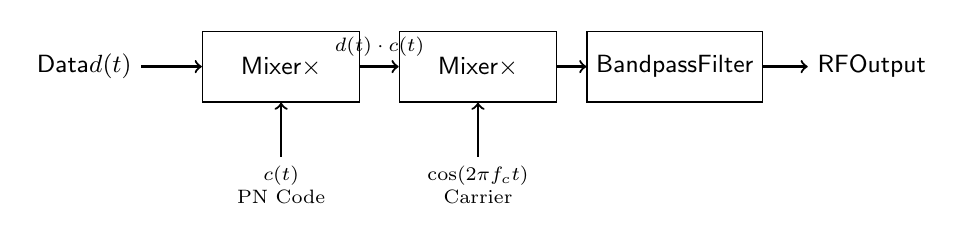
\begin{tikzpicture}[
  block/.style={rectangle, draw, minimum width=2cm, minimum height=0.9cm, font=\sffamily\small},
  node distance=2.2cm,
  font=\small
]
\node (input) {\sffamily Data\\$d(t)$};
\node[block, right of=input, node distance=2.5cm] (mult1) {Mixer\\$\times$};
\node[block, right of=mult1, node distance=2.5cm] (mult2) {Mixer\\$\times$};
\node[block, right of=mult2, node distance=2.5cm] (bpf) {Bandpass\\Filter};
\node[right of=bpf, node distance=2.5cm] (output) {\sffamily RF\\Output};

\node[below of=mult1, node distance=1.5cm, font=\scriptsize, align=center] (code) {$c(t)$\\PN Code};
\node[below of=mult2, node distance=1.5cm, font=\scriptsize, align=center] (carrier) {$\cos(2\pi f_c t)$\\Carrier};

\draw[->,thick] (input) -- (mult1);
\draw[->,thick] (code) -- (mult1);
\draw[->,thick] (mult1) -- node[above,font=\scriptsize] {$d(t) \cdot c(t)$} (mult2);
\draw[->,thick] (carrier) -- (mult2);
\draw[->,thick] (mult2) -- (bpf);
\draw[->,thick] (bpf) -- (output);
\end{tikzpicture}
\end{center}

\textbf{Process:}
\begin{enumerate}
\item \textbf{Spreading:} Multiply data $d(t)$ by high-rate PN code $c(t)$
\item \textbf{Upconversion:} Multiply by carrier to shift to RF frequency
\item \textbf{Filtering:} Bandpass filter removes out-of-band emissions
\end{enumerate}

\textbf{DSSS Receiver:}

\begin{center}
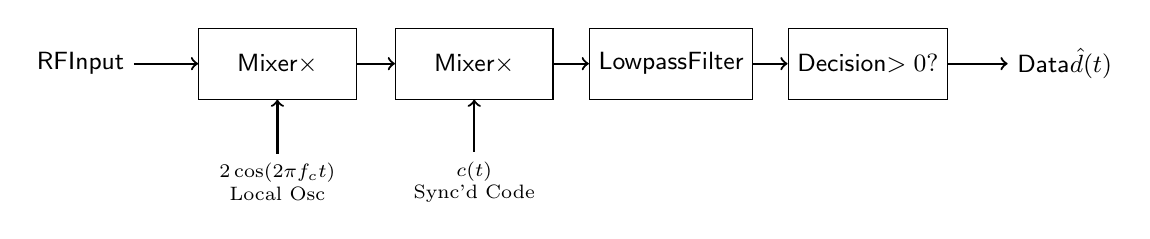
\begin{tikzpicture}[
  block/.style={rectangle, draw, minimum width=2cm, minimum height=0.9cm, font=\sffamily\small},
  node distance=2.2cm,
  font=\small
]
\node (input) {\sffamily RF\\Input};
\node[block, right of=input, node distance=2.5cm] (mult1) {Mixer\\$\times$};
\node[block, right of=mult1, node distance=2.5cm] (mult2) {Mixer\\$\times$};
\node[block, right of=mult2, node distance=2.5cm] (lpf) {Lowpass\\Filter};
\node[block, right of=lpf, node distance=2.5cm] (decide) {Decision\\$>0?$};
\node[right of=decide, node distance=2.5cm] (output) {\sffamily Data\\$\hat{d}(t)$};

\node[below of=mult1, node distance=1.5cm, font=\scriptsize, align=center] (carrier2) {$2\cos(2\pi f_c t)$\\Local Osc};
\node[below of=mult2, node distance=1.5cm, font=\scriptsize, align=center] (code2) {$c(t)$\\Sync'd Code};

\draw[->,thick] (input) -- (mult1);
\draw[->,thick] (carrier2) -- (mult1);
\draw[->,thick] (mult1) -- (mult2);
\draw[->,thick] (code2) -- (mult2);
\draw[->,thick] (mult2) -- (lpf);
\draw[->,thick] (lpf) -- (decide);
\draw[->,thick] (decide) -- (output);
\end{tikzpicture}
\end{center}

\textbf{Process:}
\begin{enumerate}
\item \textbf{Downconversion:} Multiply by local oscillator to baseband
\item \textbf{Despreading:} Multiply by synchronized PN code replica
\item \textbf{Integration:} Lowpass filter accumulates signal energy
\item \textbf{Decision:} Threshold detector recovers data bits
\end{enumerate}

\begin{warningbox}
\textbf{Code synchronization is critical.} The receiver's PN code must be aligned to within a fraction of a chip period. This requires acquisition (coarse alignment) and tracking (fine alignment) subsystems. Loss of synchronization results in complete signal loss, as the despreading process fails.
\end{warningbox}

\subsection{FHSS Frequency Hopping Pattern}

\textbf{Frequency Hopping Visualization:}

\begin{center}
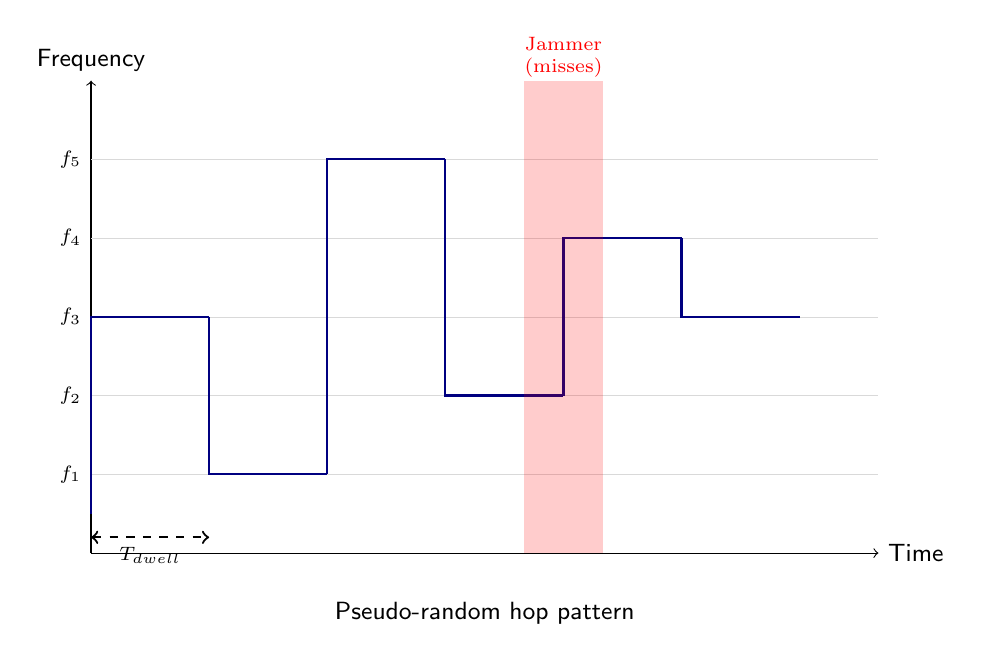
\begin{tikzpicture}[scale=1.0]
% Axes
\draw[->] (0,0) -- (10,0) node[right,font=\sffamily\small] {Time};
\draw[->] (0,0) -- (0,6) node[above,font=\sffamily\small] {Frequency};

% Frequency channels
\foreach \y in {1,2,3,4,5} {
  \draw[very thin,gray!30] (0,\y) -- (10,\y);
  \node[left,font=\scriptsize] at (0,\y) {$f_{\y}$};
}

% Hop pattern
\draw[thick,NavyBlue] (0,0.5) -- (0,3) -- (1.5,3);
\draw[thick,NavyBlue] (1.5,3) -- (1.5,1) -- (3,1);
\draw[thick,NavyBlue] (3,1) -- (3,5) -- (4.5,5);
\draw[thick,NavyBlue] (4.5,5) -- (4.5,2) -- (6,2);
\draw[thick,NavyBlue] (6,2) -- (6,4) -- (7.5,4);
\draw[thick,NavyBlue] (7.5,4) -- (7.5,3) -- (9,3);

% Dwell time annotation
\draw[<->,thick,dashed] (0,0.2) -- (1.5,0.2) node[midway,below,font=\scriptsize] {$T_{\text{dwell}}$};

% Jammer
\fill[red,opacity=0.2] (5.5,0) rectangle (6.5,6);
\node[red,font=\scriptsize,align=center] at (6,6.3) {Jammer\\(misses)};

\node[below,font=\sffamily\small] at (5,-0.5) {Pseudo-random hop pattern};
\end{tikzpicture}
\end{center}

\textbf{Key features:}
\begin{itemize}
\item Each hop dwells for time $T_{\text{dwell}} = 1/R_{\text{hop}}$
\item Hop pattern is pseudo-random, determined by cryptographic key
\item Jammer cannot predict next frequency---must jam entire band
\item Fast hopping ($T_{\text{dwell}} < 100$ µs) defeats follower jammers
\end{itemize}

\subsection{Phased Array Beam Steering}

\textbf{Electronic Beamforming Principle:}

\begin{center}
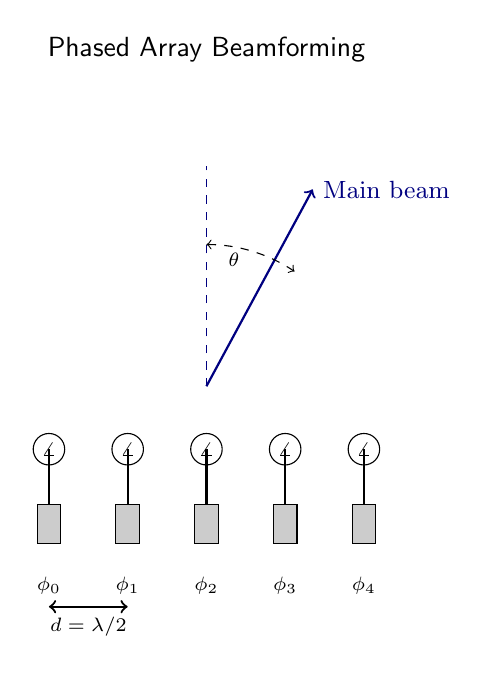
\begin{tikzpicture}[scale=1.0]
% Array elements
\foreach \x in {0,1,2,3,4} {
  \draw[fill=black!20] (\x,0) rectangle (\x+0.3,0.5);
  \node[below,font=\scriptsize] at (\x+0.15,-0.3) {$\phi_{\x}$};
}

% Phase shifters
\foreach \x in {0,1,2,3,4} {
  \draw[thick] (\x+0.15,0.5) -- (\x+0.15,1.2);
  \draw (\x+0.15,1.2) circle (0.2);
  \node[font=\tiny] at (\x+0.15,1.2) {$\angle$};
}

% Beam pattern (main lobe)
\draw[thick,NavyBlue,->] (2.15,2) -- (3.5,4.5) node[right,font=\small] {Main beam};
\draw[dashed,NavyBlue] (2.15,2) -- (2.15,4.8);

% Angle annotation
\draw[<->,dashed] (2.15,3.8) arc (90:56:2.0);
\node[font=\scriptsize] at (2.5,3.6) {$\theta$};

% Element spacing
\draw[<->,thick] (0.15,-0.8) -- (1.15,-0.8) node[midway,below,font=\scriptsize] {$d = \lambda/2$};

% Title
\node[above,font=\sffamily] at (2.15,6) {Phased Array Beamforming};
\end{tikzpicture}
\end{center}

\textbf{Beam steering equation:}
\begin{itemize}
\item Progressive phase shift: $\phi_n = (2\pi d/\lambda) n \sin(\theta)$
\item Beam angle $\theta$ controlled electronically (no mechanical motion)
\item Switching time: $<$ 1 µs (vs. seconds for mechanical scanning)
\item Multiple beams possible simultaneously (multi-target tracking)
\end{itemize}

\section{Applications}

\subsection{SATCOM Frequency Hopping (FHSS)}

In decibels:
\begin{equation}
G_{\text{dB}} = 10 \log_{10}(G)
\end{equation}

\textbf{Power Spectral Density (PSD)} after spreading:
\begin{equation}
\text{PSD} = \frac{P_{\text{TX}}}{BW_{\text{spread}}}
\end{equation}
where:
\begin{itemize}
\item $P_{\text{TX}}$ = transmit power (W)
\item PSD = power per unit bandwidth (W/Hz)
\end{itemize}

\begin{calloutbox}{LPD Threshold}
For LPD, the signal PSD must be below the thermal noise floor. With processing gain $G > 30$~dB (factor of 1000), the spread signal becomes indistinguishable from background noise to wideband receivers.
\end{calloutbox}

\subsection{Jamming Margin}

The ability to overcome jamming is quantified by the \textbf{jamming margin}:
\begin{equation}
M_{\text{jam}} = G_{\text{dB}} - \frac{J}{S} - \left(\frac{E_b}{N_0}\right)_{\text{req}} - L
\end{equation}
where:
\begin{itemize}
\item $M_{\text{jam}}$ = jamming margin (dB), positive = link survives
\item $J/S$ = jammer-to-signal ratio at receiver (dB)
\item $(E_b/N_0)_{\text{req}}$ = required bit energy to noise ratio (dB)
\item $L$ = implementation losses (dB)
\end{itemize}

\begin{warningbox}
A positive jamming margin is essential for link survival. Military systems typically design for $M_{\text{jam}} \geq 10$~dB to account for fading and worst-case scenarios.
\end{warningbox}

\section{SATCOM Frequency Hopping (FHSS)}

Military satellite communications use Frequency Hopping Spread Spectrum (FHSS) for transmission security (TRANSEC) and anti-jamming.

\subsection{MILSTAR System Parameters}

\textbf{MILSTAR (Military Strategic and Tactical Relay)} specifications:
\begin{itemize}
\item Frequency: X-band uplink (7--8~GHz), Ka-band downlink (20--21~GHz)
\item Hop rate: 100--1000+ hops/second
\item Hop set: 1000+ frequencies across 1~GHz bandwidth
\item Dwell time: $<1$~ms per hop
\item Modulation: BPSK, QPSK, 8-PSK (adaptive)
\item Data rate: 75~bps to 1.544~Mbps
\item Constellation: 5 GEO satellites (global coverage)
\end{itemize}

\subsection{FHSS Processing Gain}

For frequency hopping, the processing gain is:
\begin{equation}
G_{\text{FH}} = N_{\text{hop}}
\end{equation}
where:
\begin{itemize}
\item $N_{\text{hop}}$ = number of frequencies in hop set
\end{itemize}

In decibels:
\begin{equation}
G_{\text{FH,dB}} = 10 \log_{10}(N_{\text{hop}})
\end{equation}

For MILSTAR with $N_{\text{hop}} = 1000$:
\begin{equation}
G_{\text{FH,dB}} = 10 \log_{10}(1000) = 30 \text{ dB}
\end{equation}

\subsection{LPI/LPD Analysis}

The power spectral density after frequency spreading:
\begin{equation}
\text{PSD} = \frac{P_{\text{TX}}}{BW_{\text{hop set}}}
\end{equation}

For MILSTAR ($P_{\text{TX}} = 100$~W, $BW_{\text{hop set}} = 1$~GHz):
\begin{equation}
\text{PSD} = \frac{100 \text{ W}}{10^9 \text{ Hz}} = 10^{-7} \text{ W/Hz} = -70 \text{ dBm/Hz}
\end{equation}

Thermal noise floor at 1~MHz bandwidth:
\begin{equation}
N = -174 \text{ dBm/Hz} + 10 \log_{10}(10^6) = -114 \text{ dBm/MHz}
\end{equation}

\begin{keyconcept}
The signal PSD ($-70$~dBm/MHz) is below the noise floor ($-114$~dBm/MHz when integrated over 1~MHz). This makes the transmission undetectable to wideband receivers without knowledge of the hopping pattern.
\end{keyconcept}

\subsection{Frequency Hopping Pattern Visualization}

\begin{center}
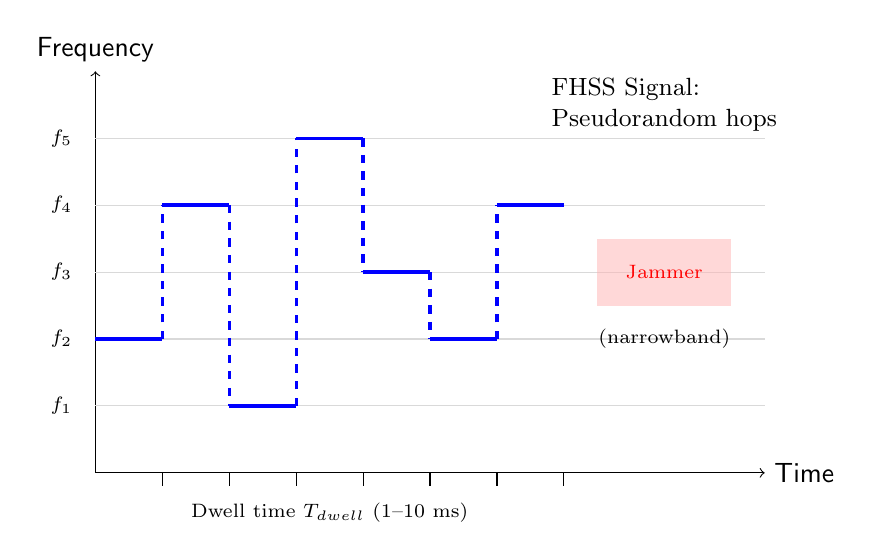
\begin{tikzpicture}[scale=0.85]
% Axes
\draw[->] (0,0) -- (10,0) node[right] {\sffamily Time};
\draw[->] (0,0) -- (0,6) node[above] {\sffamily Frequency};

% Frequency levels
\foreach \y in {1,2,3,4,5} {
  \draw[thin,gray!30] (0,\y) -- (10,\y);
  \node[left,font=\scriptsize] at (-0.2,\y) {$f_{\y}$};
}

% Hopping pattern (example sequence)
\draw[very thick,blue] (0,2) -- (1,2);
\draw[very thick,blue,dashed] (1,2) -- (1,4);
\draw[very thick,blue] (1,4) -- (2,4);
\draw[very thick,blue,dashed] (2,4) -- (2,1);
\draw[very thick,blue] (2,1) -- (3,1);
\draw[very thick,blue,dashed] (3,1) -- (3,5);
\draw[very thick,blue] (3,5) -- (4,5);
\draw[very thick,blue,dashed] (4,5) -- (4,3);
\draw[very thick,blue] (4,3) -- (5,3);
\draw[very thick,blue,dashed] (5,3) -- (5,2);
\draw[very thick,blue] (5,2) -- (6,2);
\draw[very thick,blue,dashed] (6,2) -- (6,4);
\draw[very thick,blue] (6,4) -- (7,4);

% Time slots
\foreach \x in {1,2,3,4,5,6,7} {
  \draw[thin] (\x,0) -- (\x,-0.2);
}
\node[below,font=\scriptsize] at (3.5,-0.3) {Dwell time $T_{\text{dwell}}$ (1--10 ms)};

% Jammer illustration
\fill[red!30,opacity=0.5] (7.5,2.5) rectangle (9.5,3.5);
\node[font=\scriptsize,red] at (8.5,3) {Jammer};
\node[font=\scriptsize] at (8.5,2) {(narrowband)};

% Legend
\node[font=\small,align=left] at (8.5,5.5) {FHSS Signal:\\Pseudorandom hops};

\end{tikzpicture}
\end{center}

\textbf{Cryptographic synchronization:}
\begin{itemize}
\item Hopping pattern generated by NSA-approved algorithm
\item Synchronized using GPS time + Key Encryption Key (KEK)
\item Pattern period: days to weeks (appears never-repeating)
\end{itemize}

\subsection{FHSS Anti-Jam Performance}

\textbf{Scenario:} Tactical UHF link under jamming.

\textbf{Given parameters:}
\begin{itemize}
\item Processing gain: $G = 30$~dB (1000 hop set)
\item Jammer-to-signal ratio: $J/S = 40$~dB (jammer 10,000$\times$ stronger)
\item Required $E_b/N_0$: 10~dB (BPSK, BER $= 10^{-5}$)
\item Implementation losses: $L = 3$~dB
\end{itemize}

\textbf{Initial jamming margin:}
\begin{equation}
M_{\text{jam}} = 30 - 40 - 10 - 3 = -23 \text{ dB} \quad \text{(LINK FAILS)}
\end{equation}

\textbf{Countermeasure 1 -- Directional antenna:}
\begin{itemize}
\item Gain toward satellite: $+20$~dB
\item Null toward jammer: $-20$~dB
\item Effective $J/S = 40 - 20 = 20$~dB
\end{itemize}
\begin{equation}
M_{\text{jam}} = 30 - 20 - 10 - 3 = -3 \text{ dB} \quad \text{(MARGINAL)}
\end{equation}

\textbf{Countermeasure 2 -- Forward error correction:}
\begin{itemize}
\item Turbo/LDPC code rate-1/3: $+5$~dB coding gain
\end{itemize}
\begin{equation}
M_{\text{jam}} = -3 + 5 = +2 \text{ dB} \quad \text{(LINK SURVIVES)}
\end{equation}

\begin{calloutbox}{Layered Defense}
Military systems combine multiple anti-jam techniques: spread spectrum processing gain, directional antennas with nulling, forward error correction, and burst transmission. Each layer adds 3--20~dB of protection.
\end{calloutbox}

\subsection{Follower Jamming Resistance}

\textbf{Threat:} Smart jammer detects hop and jams that frequency.

Timing analysis for follower jammer defeat:
\begin{equation}
T_{\text{effective jam}} = T_{\text{dwell}} - (T_{\text{detect}} + T_{\text{switch}})
\end{equation}
where:
\begin{itemize}
\item $T_{\text{dwell}}$ = dwell time per frequency (ms)
\item $T_{\text{detect}}$ = jammer detection time ($\mu$s)
\item $T_{\text{switch}}$ = jammer frequency switching time ($\mu$s)
\end{itemize}

\textbf{Example -- MILSTAR defense:}
\begin{itemize}
\item Dwell time: $T_{\text{dwell}} = 1$~ms
\item Jammer detection: $T_{\text{detect}} = 100~\mu$s
\item Jammer switching: $T_{\text{switch}} = 50~\mu$s
\item Total jammer delay: $150~\mu$s
\end{itemize}
\begin{equation}
T_{\text{effective jam}} = 1000~\mu\text{s} - 150~\mu\text{s} = 850~\mu\text{s} \quad (85\% \text{ of hop})
\end{equation}

\textbf{Countermeasure -- Fast hopping:}
\begin{itemize}
\item Reduce dwell time: $T_{\text{dwell}} = 100~\mu$s (10$\times$ faster)
\end{itemize}
\begin{equation}
T_{\text{effective jam}} = 100~\mu\text{s} - 150~\mu\text{s} < 0 \quad \text{(jammer too slow!)}
\end{equation}

Modern military systems use $T_{\text{dwell}} = 10$--$100~\mu$s to defeat follower jammers.

\section{GPS M-Code (Military GPS)}

GPS Modernization provides jam-resistant, encrypted positioning for military users through M-code.

\subsection{Signal Structure}

\textbf{GPS L1 M-Code parameters:}
\begin{itemize}
\item Carrier frequency: $f_c = 1575.42$~MHz (L1 band)
\item Chip rate: $R_c = 5.115$~Mcps (5$\times$ faster than C/A code)
\item Code length: Classified (estimated $\sim 10^{13}$ chips, never repeats)
\item Modulation: BOC(10,5) -- Binary Offset Carrier
\item Processing gain: $\sim 50$~dB (vs. 43~dB for C/A)
\item Power: 6.5~dB stronger than C/A code
\item Security: Encrypted, NSA-authenticated
\end{itemize}

\textbf{GPS L2 M-Code:}
\begin{itemize}
\item Carrier frequency: $f_c = 1227.60$~MHz (L2 band)
\item Same structure as L1 M-code
\item Dual-frequency enables ionospheric correction
\end{itemize}

\subsection{BOC Modulation}

Binary Offset Carrier (BOC) modulates the chip sequence with a square wave subcarrier. For BOC($m$, $n$):
\begin{equation}
s(t) = \text{sign}[\sin(2\pi f_{\text{sub}} t)] \cdot c(t) \cdot \cos(2\pi f_c t)
\end{equation}
where:
\begin{itemize}
\item $f_{\text{sub}} = m \times 1.023$~MHz = subcarrier frequency
\item $c(t) = \pm 1$ = spreading code at rate $n \times 1.023$~Mcps
\item $m = 10$, $n = 5$ for GPS M-code
\end{itemize}

For BOC(10,5):
\begin{equation}
f_{\text{sub}} = 10 \times 1.023 \text{ MHz} = 10.23 \text{ MHz}
\end{equation}
\begin{equation}
R_c = 5 \times 1.023 \text{ Mcps} = 5.115 \text{ Mcps}
\end{equation}

\begin{calloutbox}{Split-Spectrum Design}
BOC(10,5) splits power into upper and lower sidebands at $f_c \pm 10.23$~MHz. This minimizes interference with civilian C/A code (centered at $f_c$) while providing better multipath rejection and ranging accuracy.
\end{calloutbox}

\subsection{GPS M-Code Anti-Jam Performance}

\textbf{Scenario 1 -- Wideband barrage jamming:}

\textbf{Given:}
\begin{itemize}
\item Received signal power (M-code): $P_s = -163$~dBW
\item Jammer power at receiver: $P_j = -100$~dBW (50~km distance)
\item Processing gain: $G = 50$~dB
\item Required $E_b/N_0 = 10$~dB
\end{itemize}

Jammer-to-signal ratio:
\begin{equation}
J/S = P_j - P_s = -100 - (-163) = 63 \text{ dB}
\end{equation}

Initial jamming margin:
\begin{equation}
M_{\text{jam}} = 50 - 63 - 10 = -23 \text{ dB} \quad \text{(LINK FAILS)}
\end{equation}

\textbf{Binary Offset Carrier (BOC)} modulates the chip sequence with a square wave subcarrier, creating a split-spectrum signature that improves multipath rejection and coexistence with C/A code.

\textbf{BOC(m,n) notation:}
\begin{itemize}
\item $m$ = subcarrier frequency multiplier (MHz)
\item $n$ = chip rate multiplier (MHz)
\end{itemize}

For BOC(10,5):
\begin{equation}
f_{\text{sub}} = 10.23 \text{ MHz} \quad \text{(2$\times$ C/A chip rate)}
\end{equation}
\begin{equation}
R_{\text{chip}} = 5.115 \text{ Mcps} \quad \text{(5$\times$ C/A chip rate)}
\end{equation}

\textbf{BOC Modulation Spectrum:}

\begin{center}
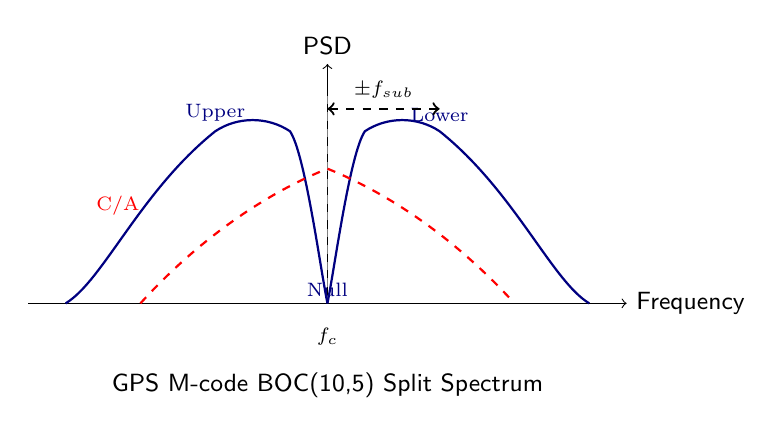
\begin{tikzpicture}[scale=0.95]
% Axes
\draw[->] (-4,0) -- (4,0) node[right,font=\sffamily\small] {Frequency};
\draw[->] (0,0) -- (0,3.2) node[above,font=\sffamily\small] {PSD};

% Center frequency marker
\draw[dashed,gray] (0,0) -- (0,2.8);
\node[below,font=\scriptsize] at (0,-0.2) {$f_c$};

% BOC split spectrum (two main lobes)
\draw[thick,NavyBlue] (-3.5,0) .. controls (-3,0.3) and (-2.5,1.5) .. (-1.5,2.3) 
  .. controls (-1.2,2.5) and (-0.8,2.5) .. (-0.5,2.3)
  .. controls (-0.3,2.0) and (-0.1,0.5) .. (0,0);
\draw[thick,NavyBlue] (0,0) .. controls (0.1,0.5) and (0.3,2.0) .. (0.5,2.3)
  .. controls (0.8,2.5) and (1.2,2.5) .. (1.5,2.3)
  .. controls (2.5,1.5) and (3,0.3) .. (3.5,0);

% Peak labels
\node[above,font=\scriptsize,NavyBlue] at (-1.5,2.3) {Upper};
\node[above,font=\scriptsize,NavyBlue] at (1.5,2.3) {Lower};

% Frequency offset annotation
\draw[<->,thick,dashed] (0,2.6) -- (1.5,2.6) node[midway,above,font=\scriptsize] {$\pm f_{\text{sub}}$};

% C/A code spectrum (for comparison)
\draw[thick,red,dashed] (-2.5,0) .. controls (-1.5,1.1) and (-0.5,1.6) .. (0,1.8)
  .. controls (0.5,1.6) and (1.5,1.1) .. (2.5,0);
\node[red,font=\scriptsize] at (-2.8,1.3) {C/A};

% Null at center
\node[below,font=\scriptsize,NavyBlue] at (0,0.4) {Null};

\node[below,font=\sffamily\small] at (0,-0.8) {GPS M-code BOC(10,5) Split Spectrum};
\end{tikzpicture}
\end{center}

\textbf{BOC signal equation:}
\begin{equation}
s_{\text{BOC}}(t) = \text{sign}[\sin(2\pi f_{\text{sub}} t)] \cdot c(t) \cdot \cos(2\pi f_c t)
\end{equation}
where:
\begin{itemize}
\item $\text{sign}[\cdot]$ = square wave subcarrier ($\pm 1$)
\item $c(t)$ = spreading code
\item $f_c$ = carrier frequency (L1: 1575.42 MHz)
\end{itemize}

\textbf{Advantages of BOC:}
\begin{itemize}
\item Split spectrum reduces interference with C/A code at $f_c$
\item Sharper autocorrelation improves ranging accuracy
\item Higher bandwidth provides multipath rejection
\item Processing gain: $\sim 50$ dB (vs. 43 dB for C/A code)
\end{itemize}

\textbf{Power and Processing Gain:}
\begin{equation}
G_{\text{M-code}} = 10\log_{10}\left(\frac{f_{\text{sub}}}{R_{\text{bit}}}\right) \approx 50 \text{ dB}
\end{equation}
where:
\begin{itemize}
\item M-code is 6.5 dB stronger than C/A code in received power
\item Combined with processing gain, provides $>$ 55 dB jamming margin
\end{itemize}

\textbf{Time-domain visualization:}

For an $N$-element linear array with element spacing $d$, the phase shift required to steer the beam to angle $\theta$ is:
\begin{equation}
\phi_n = \frac{2\pi}{\lambda} d \sin(\theta) \cdot n
\end{equation}
where:
\begin{itemize}
\item $\phi_n$ = phase shift for element $n$ (radians)
\item $\lambda$ = wavelength (m)
\item $d$ = element spacing (m)
\item $\theta$ = beam steering angle from broadside (degrees)
\item $n = 0, 1, 2, \ldots, N-1$ = element index
\end{itemize}

\textbf{Example -- 8-element array, $d = \lambda/2$, steer to $\theta = 30°$:}
\begin{equation}
\phi_n = \frac{2\pi}{\lambda} \cdot \frac{\lambda}{2} \cdot \sin(30°) \cdot n = \frac{\pi}{2} \cdot n = 90° \cdot n
\end{equation}

Element phases: $[0°, 90°, 180°, 270°, 0°, 90°, 180°, 270°]$

\subsection{Phased Array Beamforming Visualization}

\begin{center}
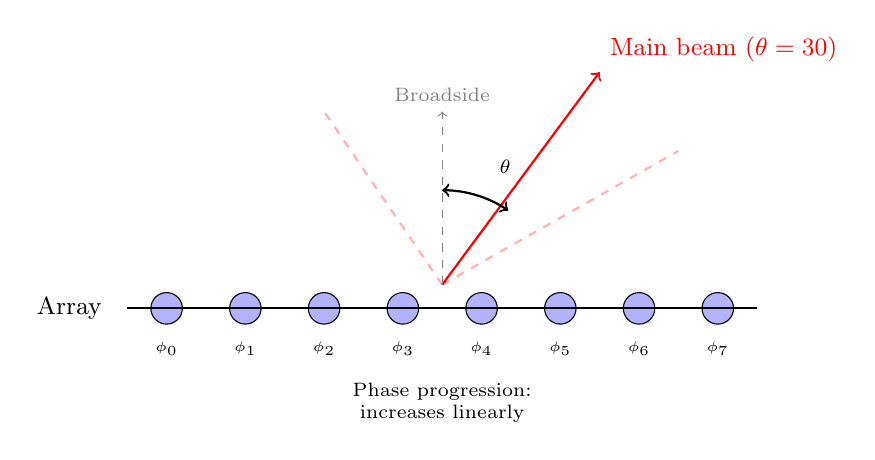
\begin{tikzpicture}[scale=1.0]
% Array elements
\foreach \x in {0,1,2,3,4,5,6,7} {
  \draw[fill=blue!30] (\x,0) circle (0.2);
  \node[below,font=\tiny] at (\x,-0.3) {$\phi_{\x}$};
}

% Array line
\draw[thick] (-0.5,0) -- (7.5,0);
\node[left,font=\small] at (-0.7,0) {Array};

% Beam pattern (simplified)
\draw[red,thick,->] (3.5,0.3) -- (5.5,3) node[above right,font=\small] {Main beam ($\theta = 30°$)};
\draw[red,thick,dashed,opacity=0.3] (3.5,0.3) -- (2,2.5);
\draw[red,thick,dashed,opacity=0.3] (3.5,0.3) -- (6.5,2);

% Broadside reference
\draw[gray,dashed,->] (3.5,0.3) -- (3.5,2.5) node[above,font=\scriptsize,gray] {Broadside};

% Angle annotation
\draw[<->,thick] (3.5,1.5) arc (90:56:1.5);
\node[font=\scriptsize] at (4.3,1.8) {$\theta$};

% Phase progression
\node[font=\scriptsize,align=center] at (3.5,-1.2) {Phase progression:\\increases linearly};

\end{tikzpicture}
\end{center}

\subsection{Array Performance Parameters}

\textbf{Array gain:}
\begin{equation}
G_{\text{array}} = N \cdot G_{\text{element}}
\end{equation}

In decibels:
\begin{equation}
G_{\text{array,dB}} = 10 \log_{10}(N) + G_{\text{element,dB}}
\end{equation}

For 256-element AESA with $G_{\text{element}} = 5$~dBi:
\begin{equation}
G_{\text{array,dB}} = 10 \log_{10}(256) + 5 = 24 + 5 = 29 \text{ dBi}
\end{equation}

\textbf{Beamwidth (half-power):}
\begin{equation}
\theta_{3\text{dB}} \approx \frac{\lambda}{N \cdot d} \quad \text{(radians)}
\end{equation}

For 256 elements with $d = \lambda/2$:
\begin{equation}
\theta_{3\text{dB}} \approx \frac{\lambda}{256 \cdot \lambda/2} = \frac{1}{128} \text{ rad} \approx 0.45°
\end{equation}

\begin{calloutbox}{LPI Advantage}
Narrow beamwidth ($<1°$) concentrates radiated power in a small solid angle, making the signal difficult to intercept from off-axis directions. Combined with low peak power and frequency agility, AESA radars achieve excellent LPI performance.
\end{calloutbox}

\subsection{AESA Applications}

\textbf{APG-77 (F-22 Raptor):}
\begin{itemize}
\item Frequency: X-band (8--12~GHz), 4~GHz agility
\item Array: 2000+ transmit/receive (T/R) modules
\item Power: 13~kW average, 20~kW peak per module
\item Modes: Air-to-air, air-to-ground, SAR, electronic attack
\item Detection range: $>200$~km (fighter-sized target)
\item LPI: Adaptive power, narrow beamwidth (1--2°), low sidelobes ($<-40$~dB)
\end{itemize}

\textbf{AN/SPY-6 (U.S. Navy DDG-51):}
\begin{itemize}
\item Frequency: S-band (3.3--3.5~GHz)
\item Array: 37 Radar Modular Assemblies (RMAs), 5000+ T/R modules
\item Power: 6~MW average radiated power
\item Range: $>300$~km (ballistic missile detection)
\item Capabilities: Track 1000+ targets, adaptive nulling, multi-mission
\end{itemize}

\section{Link 16 (JTIDS)}

Joint Tactical Information Distribution System provides jam-resistant, LPI/LPD tactical data networking.

\subsection{Network Architecture}

\textbf{Participants:}
\begin{itemize}
\item Aircraft: F-15, F-16, F-22, F-35, E-3 AWACS
\item Ships: Aegis cruisers/destroyers, carriers
\item Ground: Patriot SAM, THAAD, command posts
\end{itemize}

\textbf{Topology:} Time Division Multiple Access (TDMA)
\begin{itemize}
\item 128 time slots per 12-second frame
\item Nodes assigned slots (voice/data)
\item Collision-free multiple access
\end{itemize}

\subsection{Link 16 Network Topology}

\begin{center}
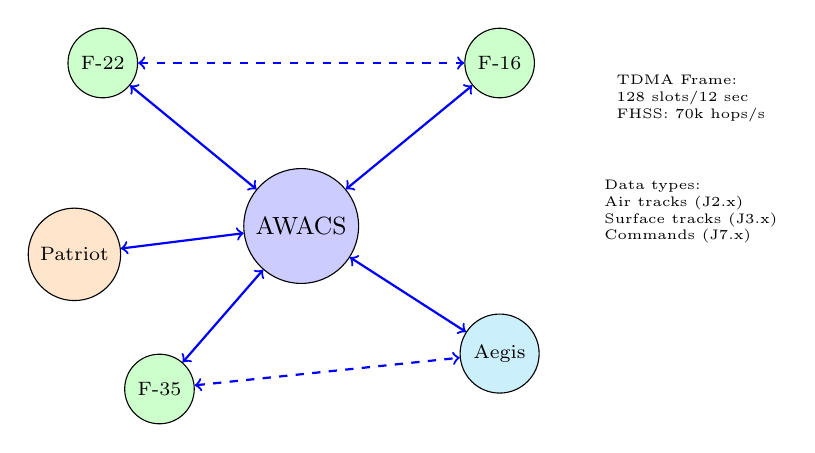
\begin{tikzpicture}[scale=0.9]
% Central node (AWACS)
\node[circle,draw,fill=blue!20,minimum size=1.1cm,font=\small] (awacs) at (0,0) {AWACS};

% Fighter nodes
\node[circle,draw,fill=green!20,minimum size=0.85cm,font=\scriptsize] (f22) at (-2.8,2.3) {F-22};
\node[circle,draw,fill=green!20,minimum size=0.85cm,font=\scriptsize] (f16) at (2.8,2.3) {F-16};
\node[circle,draw,fill=green!20,minimum size=0.85cm,font=\scriptsize] (f35) at (-2,-2.3) {F-35};

% Ship node
\node[circle,draw,fill=cyan!20,minimum size=0.85cm,font=\scriptsize] (aegis) at (2.8,-1.8) {Aegis};

% Ground node
\node[circle,draw,fill=orange!20,minimum size=0.85cm,font=\scriptsize] (patriot) at (-3.2,-0.4) {Patriot};

% Connections (bidirectional)
\draw[<->,thick,blue] (awacs) -- (f22);
\draw[<->,thick,blue] (awacs) -- (f16);
\draw[<->,thick,blue] (awacs) -- (f35);
\draw[<->,thick,blue] (awacs) -- (aegis);
\draw[<->,thick,blue] (awacs) -- (patriot);
\draw[<->,thick,blue,dashed] (f22) -- (f16);
\draw[<->,thick,blue,dashed] (f35) -- (aegis);

% Legend
\node[align=left,font=\tiny] at (5.5,1.8) {TDMA Frame:\\128 slots/12 sec\\FHSS: 70k hops/s};
\node[align=left,font=\tiny] at (5.5,0.2) {Data types:\\Air tracks (J2.x)\\Surface tracks (J3.x)\\Commands (J7.x)};

\end{tikzpicture}
\end{center}

\subsection{Link 16 Waveform Parameters}

\textbf{Physical layer:}
\begin{itemize}
\item Frequency: 960--1215~MHz (L-band)
\item Modulation: MSK (Minimum Shift Keying) -- constant envelope
\item Waveform: FHSS + TDMA hybrid
\item Hop rate: 70,000 hops/second
\item Hop duration: $\sim 14~\mu$s
\item Channels: 51 frequencies (15~MHz spacing)
\item Data rate: 28.8~kbps (typical), up to 115.2~kbps
\end{itemize}

\subsection{Link 16 Processing Gain}

Combined FHSS and TDMA provide multi-layer processing gain:
\begin{equation}
G_{\text{total}} = G_{\text{FH}} + G_{\text{TDMA}}
\end{equation}

Frequency hopping gain:
\begin{equation}
G_{\text{FH,dB}} = 10 \log_{10}(51) = 17 \text{ dB}
\end{equation}

Time diversity gain:
\begin{equation}
G_{\text{TDMA,dB}} = 10 \log_{10}(128) = 21 \text{ dB}
\end{equation}

Total processing gain:
\begin{equation}
G_{\text{total}} = 17 + 21 = 38 \text{ dB}
\end{equation}

\subsection{TRANSEC and Synchronization}

\textbf{Cryptographic hopping pattern generation:}
\begin{itemize}
\item Input: Network ID + GPS time + Crypto key (KY-58/KG-84)
\item Output: Pseudorandom frequency sequence
\item Pattern period: Classified (days to months, appears never-repeating)
\item Synchronization: GPS time $\pm 100~\mu$s accuracy required
\item Anti-spoofing: Time-of-Transmission (TOT) authentication
\end{itemize}

\section{Worked Example: Link 16 Jamming Margin}

\textbf{Problem:} Calculate the jamming margin for a Link 16 tactical data link under enemy jamming.

\textbf{Given:}
\begin{itemize}
\item Processing gain: $G = 38$~dB (FHSS + TDMA)
\item Jammer-to-signal ratio: $J/S = 50$~dB (jammer 100~km away)
\item Required $E_b/N_0 = 12$~dB (MSK with FEC)
\item Implementation losses: $L = 3$~dB
\end{itemize}

\textbf{Required:} Determine if link survives and identify countermeasures.

\textbf{Solution:}

\textit{Step 1: Calculate initial jamming margin.}

Using Equation~(4):
\begin{equation}
M_{\text{jam}} = G - J/S - (E_b/N_0)_{\text{req}} - L
\end{equation}
\begin{equation}
M_{\text{jam}} = 38 - 50 - 12 - 3 = -27 \text{ dB}
\end{equation}

\textbf{Result:} $M_{\text{jam}} < 0$ --- LINK FAILS.

\textit{Step 2: Apply directional antenna countermeasure.}
\begin{itemize}
\item Antenna gain toward participant: $+10$~dBi
\item Null depth toward jammer: $-20$~dB
\item Front-to-back ratio: 30~dB
\end{itemize}

Effective jammer-to-signal ratio:
\begin{equation}
J/S_{\text{effective}} = 50 - 30 = 20 \text{ dB}
\end{equation}

Revised jamming margin:
\begin{equation}
M_{\text{jam}} = 38 - 20 - 12 - 3 = 3 \text{ dB}
\end{equation}

\textbf{Answer:} With directional antenna, $M_{\text{jam}} = +3$~dB --- LINK SURVIVES.

\textbf{Interpretation:} The 3~dB margin provides minimal protection. For robust operation, additional countermeasures such as adaptive power control or higher-gain antennas would be recommended to achieve $M_{\text{jam}} \geq 10$~dB.

\section{Covert Communications}

\subsection{Objective}

Transmit data undetected by adversary signals intelligence (SIGINT) systems through Low Probability of Detection (LPD) techniques.

\subsection{Ultra-Wideband Spread Spectrum}

For covert communications, ultra-wideband (UWB) spread spectrum achieves LPD by spreading the signal power so thinly that it appears as thermal noise.

\textbf{Example parameters:}
\begin{itemize}
\item Data rate: $R_b = 1$~kbps
\item Spread bandwidth: $BW = 1$~GHz
\item Transmit power: $P_{TX} = 1$~W
\end{itemize}

Processing gain:
\begin{equation}
G = \frac{BW}{R_b} = \frac{10^9}{10^3} = 10^6 \quad (60 \text{ dB})
\end{equation}

Transmitted power spectral density:
\begin{equation}
\text{PSD} = \frac{P_{TX}}{BW} = \frac{1 \text{ W}}{10^9 \text{ Hz}} = 10^{-9} \text{ W/Hz} = -90 \text{ dBm/Hz}
\end{equation}

Per MHz:
\begin{equation}
\text{PSD}_{\text{MHz}} = -90 + 10 \log_{10}(10^6) = -30 \text{ dBm/MHz}
\end{equation}

Thermal noise floor (per MHz):
\begin{equation}
N_{\text{MHz}} = -174 \text{ dBm/Hz} + 10 \log_{10}(10^6) = -114 \text{ dBm/MHz}
\end{equation}

\begin{keyconcept}
The signal PSD ($-90$~dBm/Hz) is 24~dB below the thermal noise floor ($-114$~dBm/MHz when integrated over 1~MHz). Even sensitive intercept receivers cannot distinguish the transmission from background noise without knowledge of the spreading code and precise synchronization.
\end{keyconcept}

\subsection{Spread Spectrum Below Noise Floor Visualization}

\begin{center}
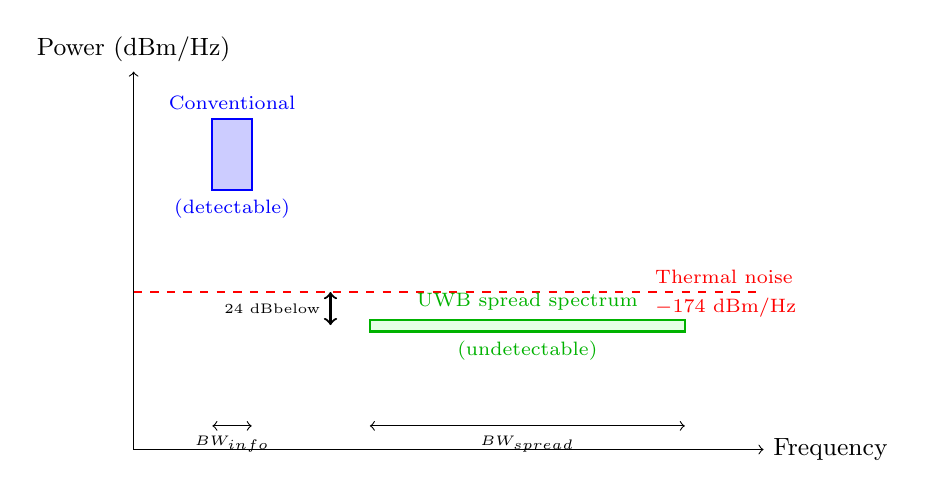
\begin{tikzpicture}[scale=1.0]
% Axes
\draw[->] (0,0) -- (8,0) node[right,font=\small] {Frequency};
\draw[->] (0,0) -- (0,4.8) node[above,font=\small] {Power (dBm/Hz)};

% Noise floor
\draw[thick,red,dashed] (0,2) -- (8,2);
\node[right,font=\scriptsize,red] at (6.5,2.2) {Thermal noise};
\node[right,font=\scriptsize,red] at (6.5,1.8) {$-174$ dBm/Hz};

% Narrowband signal (conventional)
\draw[thick,blue,fill=blue!20] (1,4.2) rectangle (1.5,3.3);
\node[above,font=\scriptsize,blue] at (1.25,4.2) {Conventional};
\node[below,font=\scriptsize,blue] at (1.25,3.3) {(detectable)};

% Spread spectrum signal (below noise)
\draw[thick,green!70!black,fill=green!10] (3,1.5) rectangle (7,1.65);
\node[above,font=\scriptsize,green!70!black] at (5,1.65) {UWB spread spectrum};
\node[below,font=\scriptsize,green!70!black] at (5,1.5) {(undetectable)};

% Annotations
\draw[<->,thick] (2.5,1.58) -- (2.5,2) node[midway,left,font=\tiny] {24 dB\\below};

% Bandwidth indicators
\draw[<->,thin] (1,0.3) -- (1.5,0.3) node[midway,below,font=\tiny] {$BW_{\text{info}}$};
\draw[<->,thin] (3,0.3) -- (7,0.3) node[midway,below,font=\tiny] {$BW_{\text{spread}}$};

\end{tikzpicture}
\end{center}

\subsection{Additional Covert Techniques}

\textbf{Steganography in OFDM:}
\begin{itemize}
\item Hide data in unused subcarriers or modulate pilot tone phases
\item OFDM pilot modulation: Covert channel up to 1~Mbps (802.11a)
\item Null subcarrier insertion: Low-power data on reserved frequencies
\item Detection challenge: Requires statistical analysis or wideband monitoring
\end{itemize}

\textbf{Time-domain hiding:}
\begin{itemize}
\item Insert ultra-short bursts in inter-frame gaps (e.g., WiFi SIFS)
\item Covert capacity: $\sim 6$~Mbps using 6.25\% duty cycle
\item Detection: Appears as multipath or transient interference
\end{itemize}

\section{Applications}

\subsection{GPS M-Code}

\textbf{Systems:} JDAM precision bombs, Tomahawk cruise missiles, Excalibur artillery, fighter avionics (F-22, F-35, B-2)

\textbf{Performance:}
\begin{itemize}
\item Positioning accuracy: $<1$~m horizontal, $<3$~m vertical
\item Time accuracy: $<10$~ns (critical for network synchronization)
\item Anti-jam: Survives 60+ dB jamming with CRPA
\end{itemize}

\subsection{MILSTAR/MUOS Satellites}

\textbf{Systems:} Strategic and tactical military satellite communications

\textbf{Capabilities:}
\begin{itemize}
\item Data rates: 75~bps to 1.544~Mbps (T1)
\item Coverage: Global (5 GEO satellites)
\item Jam resistance: 30~dB processing gain + directional antennas
\item Security: NSA Type 1 encryption
\end{itemize}

\subsection{Link 16 (JTIDS)}

\section{Worked Example: Jamming Resistance Analysis}

\textbf{Problem:} Analyze the jamming resistance of a tactical UHF SATCOM link operating under hostile conditions. Determine if the link survives when subjected to a 1 kW ground-based jammer.

\textbf{Given System Parameters:}
\begin{itemize}
\item Frequency: $f = 300$ MHz (UHF band)
\item Data rate: $R_b = 2400$ bps (digitized voice)
\item Modulation: BPSK (1 bit/symbol)
\item Spreading: DSSS with chip rate $R_c = 2.4$ Mcps
\item FEC: Rate-1/2 convolutional code (coding gain $= 5$ dB)
\item Ground terminal antenna: $G_{\text{TX}} = 10$ dBi directional
\item Transmit power: $P_{\text{TX}} = 10$ W
\item Satellite antenna: $G_{\text{RX}} = 30$ dBi
\item Distance to satellite: $d_{\text{sat}} = 40{,}000$ km (GEO)
\item Jammer power: $P_{\text{jam}} = 1$ kW
\item Jammer distance: $d_{\text{jam}} = 50$ km
\item Antenna front-to-back ratio: F/B $= 20$ dB
\end{itemize}

\textbf{Required:} Calculate the jamming margin and determine if the link operates successfully.

\textbf{Solution:}

\textit{Step 1: Calculate processing gain}

From Equation~\ref{eq:processing-gain}:
\begin{equation}
G = \frac{R_c}{R_b} = \frac{2.4 \times 10^6}{2.4 \times 10^3} = 1000
\end{equation}

In dB:
\begin{equation}
G_{\text{dB}} = 10\log_{10}(1000) = 30 \text{ dB}
\end{equation}

\textit{Step 2: Determine required $E_b/N_0$}

For BPSK at BER $= 10^{-5}$: $(E_b/N_0)_{\text{uncoded}} = 9.6$ dB

With rate-1/2 FEC coding gain of 5 dB:
\begin{equation}
\left(\frac{E_b}{N_0}\right)_{\text{req}} = 9.6 - 5 = 4.6 \text{ dB}
\end{equation}

\textit{Step 3: Calculate link budget (no jamming)}

EIRP:
\begin{equation}
\text{EIRP} = P_{\text{TX}} + G_{\text{TX}} = 40 + 10 = 50 \text{ dBm}
\end{equation}

Free-space path loss at 300 MHz, 40,000 km:
\begin{equation}
\text{FSPL} = 32.4 + 20\log_{10}(f_{\text{MHz}}) + 20\log_{10}(d_{\text{km}})
\end{equation}
\begin{equation}
\text{FSPL} = 32.4 + 20\log_{10}(300) + 20\log_{10}(40000) = 189 \text{ dB}
\end{equation}

Received signal power:
\begin{equation}
P_{\text{RX}} = \text{EIRP} - \text{FSPL} + G_{\text{RX}} = 50 - 189 + 30 = -109 \text{ dBm}
\end{equation}

Noise power in spread bandwidth:
\begin{equation}
N = -174 + 10\log_{10}(B_{\text{spread}}) = -174 + 10\log_{10}(2.4 \times 10^6) = -110 \text{ dBm}
\end{equation}

SNR:
\begin{equation}
\text{SNR} = P_{\text{RX}} - N = -109 - (-110) = 1 \text{ dB}
\end{equation}

$E_b/N_0$ after despreading:
\begin{equation}
\frac{E_b}{N_0} = \text{SNR} + G_{\text{dB}} = 1 + 30 = 31 \text{ dB}
\end{equation}

Link margin (no jamming):
\begin{equation}
M = 31 - 4.6 = 26.4 \text{ dB} \quad \checkmark \text{ (Excellent)}
\end{equation}

\textit{Step 4: Analyze jamming scenario}

Jammer path loss (300 MHz, 50 km):
\begin{equation}
\text{FSPL}_{\text{jam}} = 32.4 + 20\log_{10}(300) + 20\log_{10}(50) = 116 \text{ dB}
\end{equation}

Jammer power at receiver (no antenna discrimination):
\begin{equation}
J_{\text{RX}} = P_{\text{jam}} - \text{FSPL}_{\text{jam}} = 60 - 116 = -56 \text{ dBm}
\end{equation}

Jammer-to-signal ratio:
\begin{equation}
\frac{J}{S} = J_{\text{RX}} - P_{\text{RX}} = -56 - (-109) = 53 \text{ dB}
\end{equation}

This means the jammer is 53 dB (factor of $\sim 200{,}000$) stronger than the satellite signal!

\textit{Step 5: Apply countermeasures}

After despreading, the jammer is spread while the signal is despread:
\begin{equation}
\left(\frac{J}{S}\right)_{\text{despread}} = 53 - G_{\text{dB}} = 53 - 30 = 23 \text{ dB}
\end{equation}

Apply antenna nulling (20 dB front-to-back ratio):
\begin{equation}
\left(\frac{J}{S}\right)_{\text{effective}} = 23 - 20 = 3 \text{ dB}
\end{equation}

Effective $E_b/(N_0 + J)$:
\begin{equation}
\left(\frac{E_b}{N_0 + J}\right) = 31 - 3 = 28 \text{ dB}
\end{equation}

\textit{Step 6: Calculate jamming margin}

From Equation~\ref{eq:jamming-margin}:
\begin{equation}
M_J = 28 - 4.6 = 23.4 \text{ dB}
\end{equation}

\textbf{Answer:} The jamming margin is \textbf{+23.4 dB}. The link survives despite the jammer being 200,000 times stronger than the satellite signal.

\textbf{Interpretation:} This example demonstrates the power of combining spread spectrum (30 dB processing gain), forward error correction (5 dB coding gain), and spatial filtering (20 dB antenna nulling). Even with a 1 kW jammer at 50 km overpowering the satellite signal by 53 dB, the system maintains robust communication with over 23 dB margin. This is why GPS M-code and military SATCOM systems can operate in hostile electromagnetic environments.

\section{Performance Analysis}

\subsection{Processing Gain vs. Jamming Resistance}

The relationship between processing gain and jamming resistance is fundamental to military communications. Higher processing gain provides greater jamming margin but requires wider bandwidth.

\textbf{Key Performance Metrics:}

\begin{itemize}
\item \textbf{Jamming Margin:} $M_J = G_{\text{dB}} - (J/S)_{\text{dB}} - (E_b/N_0)_{\text{req}} - L_{\text{impl}}$
\item \textbf{LPD Threshold:} Signal PSD must be below $N_0 \approx -174$ dBm/Hz
\item \textbf{Required Processing Gain:} Depends on threat environment and link requirements
\end{itemize}

\subsection{Comparison of Military Communication Techniques}

Different military systems employ various combinations of spread spectrum, frequency hopping, and beamforming to achieve their performance goals.

\textbf{Processing Gain Comparison:}
\begin{itemize}
\item GPS C/A code: $G = 43$ dB (1.023 Mcps / 50 bps navigation data)
\item GPS M-code: $G = 50$ dB (10.23 Mcps BOC)
\item MILSTAR FHSS: $G = 30$ dB (1000 hop channels)
\item Link 16: $G = 25$ dB (FHSS + TDMA)
\item Tactical radios: $G = 20-30$ dB (typical DSSS)
\end{itemize}

\section{Summary}

Military communications systems employ a sophisticated combination of techniques to achieve robust, secure, and covert operation in hostile electromagnetic environments. The fundamental enabler is \textbf{processing gain} from spread spectrum modulation, which allows signals to operate below the noise floor while maintaining reliable links.

\textbf{Core Principles:}
\begin{itemize}
\item \textbf{Processing Gain:} $G = B_{\text{spread}}/B_{\text{info}}$ provides anti-jam capability and LPI/LPD characteristics
\item \textbf{Jamming Margin:} $M_J = G_{\text{dB}} - (J/S)_{\text{dB}} - (E_b/N_0)_{\text{req}} - L_{\text{impl}}$ quantifies link robustness
\item \textbf{LPD Threshold:} PSD must be below thermal noise floor ($N_0 \approx -174$ dBm/Hz)
\end{itemize}

\textbf{Comparison of Military Communication Techniques:}

Table~\ref{tab:military-techniques} provides a comprehensive comparison of techniques, their primary advantages, and typical applications.

\begin{table}[h]
\centering
\caption{Military Communication Techniques Comparison}
\label{tab:military-techniques}
\small
\begin{tabular}{@{}p{2.5cm}p{3cm}p{3.2cm}p{3.5cm}@{}}
\toprule
\textbf{Technique} & \textbf{Primary Gain} & \textbf{Advantage} & \textbf{Applications} \\
\midrule
DSSS & 20-40 dB proc. gain & AJ, LPI & GPS M-code, tactical radios \\
FHSS & Frequency diversity & LPD, follower-jam resistance & MILSTAR, Link 16 \\
AESA & Beamforming, agility & LPI, multi-target, EA & APG-77, AN/SPY-6 \\
Nulling Antenna & 20-40 dB spatial filter & Jammer rejection & CRPA, adaptive arrays \\
Burst TX & Temporal LPD & Minimize exposure & Submarine, UAV links \\
Encryption & Content security & Prevent exploitation & All military systems \\
Adaptive Coding & Link optimization & Maximize throughput & MUOS, 5G tactical \\
\bottomrule
\end{tabular}
\end{table}

\textbf{Key Achievements:}
\begin{itemize}
\item GPS M-code: 50 dB processing gain + BOC modulation + CRPA nulling = $>60$ dB jamming resistance
\item MILSTAR FHSS: 1000+ frequency hops across 1 GHz bandwidth, PSD below noise floor
\item AESA radars: Electronic beam steering in $<1$ µs, simultaneous multi-target tracking
\item Link 16: 70,000 hops/second with cryptographic hopping for jam-resistant tactical networking
\end{itemize}

\section{System Trade-offs}

\subsection{Disadvantages}

\begin{itemize}
\item Complexity: Requires sophisticated signal processing, synchronization
\item Cost: AESA radars and SAASM receivers are expensive
\item Bandwidth: Spread spectrum occupies wide frequency ranges
\item Latency: TDMA and hopping introduce timing delays
\item Power: Some techniques (AESA) require high transmit power
\end{itemize}

\textbf{Best suited for:} Military and government applications requiring anti-jam capability, covert operation, and secure communications in hostile electromagnetic environments.

\section{Further Reading}

\subsection{Related Chapters}

\begin{itemize}
\item Chapter~\ref{ch:spread-spectrum}: Spread Spectrum (DSSS/FHSS) -- Technical foundation for AJ/LPI
\item Chapter~\ref{ch:snr}: Signal-to-Noise Ratio (SNR) -- Link budget fundamentals
\item Chapter~\ref{ch:ber}: Bit Error Rate (BER) -- Performance analysis
\item Chapter~\ref{ch:awgn}: Additive White Gaussian Noise (AWGN) -- Channel modeling
\item Chapter~\ref{ch:fec}: Forward Error Correction (FEC) -- Coding gain
\end{itemize}

\subsection{Textbooks}

\begin{itemize}
\item \textbf{Poisel}, \emph{Introduction to Communication Electronic Warfare Systems} -- Comprehensive EW treatment
\item \textbf{Torrieri}, \emph{Principles of Spread-Spectrum Communication Systems} (4th ed.) -- Modern military focus
\item \textbf{Skolnik}, \emph{Radar Handbook} (3rd ed.) -- Phased arrays, AESA, LPI radar
\item \textbf{Adamy}, \emph{EW 101: A First Course in Electronic Warfare} -- Accessible intro to jamming/AJ
\end{itemize}

\subsection{Military Standards}

\begin{itemize}
\item \textbf{MIL-STD-188-181}: US DoD FHSS standard
\item \textbf{GPS ICD-IS-800}: M-code interface control document (FOUO)
\item \textbf{Link 16 MIDS JTIDS STD}: Message standards (NATO STANAG 5516)
\end{itemize}

\textbf{Key Takeaways:}

\begin{itemize}
\item Military communications prioritize \textbf{anti-jam (AJ)}, \textbf{LPI/LPD}, and \textbf{security (TRAN\-SEC)} over spectral efficiency
\item Processing gain from spread spectrum enables signals 20-40 dB below noise floor while maintaining robust links
\item GPS M-code combines BOC(10,5) modulation (50~dB processing gain), directional antennas (CRPA), and encryption to survive $>60$~dB jamming
\item AESA radars achieve LPI through low peak power, frequency agility, narrow beam\-widths, and electronic beam steering
\item Link 16 uses FHSS (70,000 hops/sec) with TDMA and cryptographic hopping for jam-resistant tactical data exchange
\item Jamming margin: $M_J = G_{\text{dB}} - (J/S)_{\text{dB}} - (E_b/N_0)_{\text{req}} - L_{\text{impl}}$
\item Directional antennas provide 20-40 dB additional anti-jam capability through spatial filtering
\item Modern military systems achieve \textbf{communication superiority} through layered defenses: processing gain, FEC coding, spatial filtering, and adaptive waveforms
\end{itemize}
